\documentclass[11pt,a4paper,oneside]{article}
\usepackage{P:/Latex/Config/ReadOnly/calculationReportEN}
\graphicspath{{pictures/}}
\addbibresource{P:/Latex/Config/CodesNorms.bib}
\usepackage[greek, british]{babel}
%-------------------------------------------------------------------------------------------------------------------------------------------------------------------------------------
% Defined values
% Remember to change these values below to fit the current project
%-------------------------------------------------------------------------------------------------------------------------------------------------------------------------------------



\extrafloats{500}
\newcommand{\project}{
\begin{Huge}
\color{red}{!PROJECTNAME!}
\end{Huge}
} 			%The project name for the client
\newcommand{\masterDoc}{
\begin{Huge}
\color{red}{!DOCUMENTNAME!}
\end{Huge}
} 		%The filename displayed in the footer
\newcommand{\location}{
\begin{Huge}
\color{red}{!LOCATION!}
\end{Huge}
}		%The location displayed in the report

\newcommand{\EqClass}{
\begin{Huge}
\color{red}{!EARTHQUAKE CLASS!}
\end{Huge}
} 		%The earthquake class of this project - https://asce7hazardtool.online/

\newcommand{\norm}{
\begin{Huge}
\color{red}{!NORM!}
\end{Huge}
} 		%The norm used in this project, Eurocode or ASCE // NO SPECIFICS
% For generating big tables I usually use https://www.tablesgenerator.com/
%-------------------------------------------------------------------------------------------------------------------------------------------------------------------------------------
% Begin Document
%-------------------------------------------------------------------------------------------------------------------------------------------------------------------------------------

 
\begin{document}

% The blue corner background, first page is different
\ThisURCornerWallPaper{1}{P:/Latex/Style/ENG_OmegaBlue.jpg}


% Set footer to the one used on the first page
\begin{titlepage}
\thispagestyle{fancyfirst}
\begin{figure}[H]
\vspace{-2cm}
\includegraphics[width=85mm,keepaspectratio]{P:/Latex/Style/tebulo_EN_logo.jpg}
\end{figure}
\vspace{1cm}
\begin{center}
		\Huge{\project}\\
		Design Specification\\
			
\end{center}
\iffalse
\begin{figure}[H]
\centering
\includegraphics[width=0.8\textwidth]{voorblad}
\end{figure}
\fi
%\vspace{-1cm}
%Client contact info & Logo


%Revision    

\vspace{2cm} % use this to shift the table up to accomodate more revisions, negative numbers are allowed

\Bollegraaf
% Add more revision info to the top of the table, the table automatically sits at the bottom of the page, if it doesn't fit, remove some whitespace added by the use of vspace, or just add negative whitespace by entering a negative number
\begin{table}[b]
\centering
\begin{tabular}{cccccc}
00 & First issue & J. Koning & \answerbox & \today & \answerbox\\
\hline
\textit{Rev.} & \textit{Description} & \textit{Author} & \textit{Signature Client} & \textit{Date sent} & \textit{Date signed}\\

\end{tabular}

\end{table}

\end{titlepage}


\begin{absolutelynopagebreak}
\tableofcontents

\thispagestyle{empty}

\end{absolutelynopagebreak}
% Set new corner wallpaper, and simple footer with document name (set it correctly at the top of this document, this process is not automatic!) and the page number.
\URCornerWallPaper{1}{P:/Latex/Style/ENG_volgblad_kop.jpg}
\pagestyle{fancy}
%Als er aardbevingen zijn of andere dingen binnen/buiten de standaard scope vallen, chapter 1 aanpassen
\newpage
%Make sure to fill in norm and projectname
\section{Introduction}\label{sec:Introduction}
This construction frame is designed by Tebulo Engineering according to \norm .\\
The goal of this document is to outline the requirements and demands of the construction for \project\ located in \location .
 

\newpage
%Choose between earthquake on/off
\includeversion{earthquake}
%\excludeversion{earthquake}
\section{Frame design choices}

\subsection{Support frames}
The frames are devided up into smaller phases and tags, to keep the drawings and calculations from being cluttered or confusing.\\
The support frames are generally constructed from HEA200, S235. In situations where a different profile is needed to support the loads or deal with space limitations, profiles can be chosen from HEA140 up to HEB300.\\
The wind bracings are made out of angles, 60x60x6 up to 120x120x12, in steps of 20mm.\\
The corner bracings are made out of IPE120 or IPE160, sometimes HEA profiles are chosen when necessary.\\

\subsection{Single Supports}
The columns are usually made out of UNP180.\\
The bracings are made out of flat 60x10 and angle 60x60x6.\\
There are extra angles 70x70x7 connected between the support and the conveyor, to provide stability during installment.\\
If a support is too heavily loaded, the choice can be made to construct the support from HEA.\\
 

\newpage
%If any non standard connections are to be expected, this is where you outline those
\section{Connections}

\subsection{Choosing beam and column connections}
The standard method of connecting beams to the web of the colums is to use a rigid connection, for ease of construction. Corner and wind bracings are exempt from this rule, and are mounted directly to the web, as seen in Figure \ref{fig:cornerBracing}.


\begin{figure}[H]
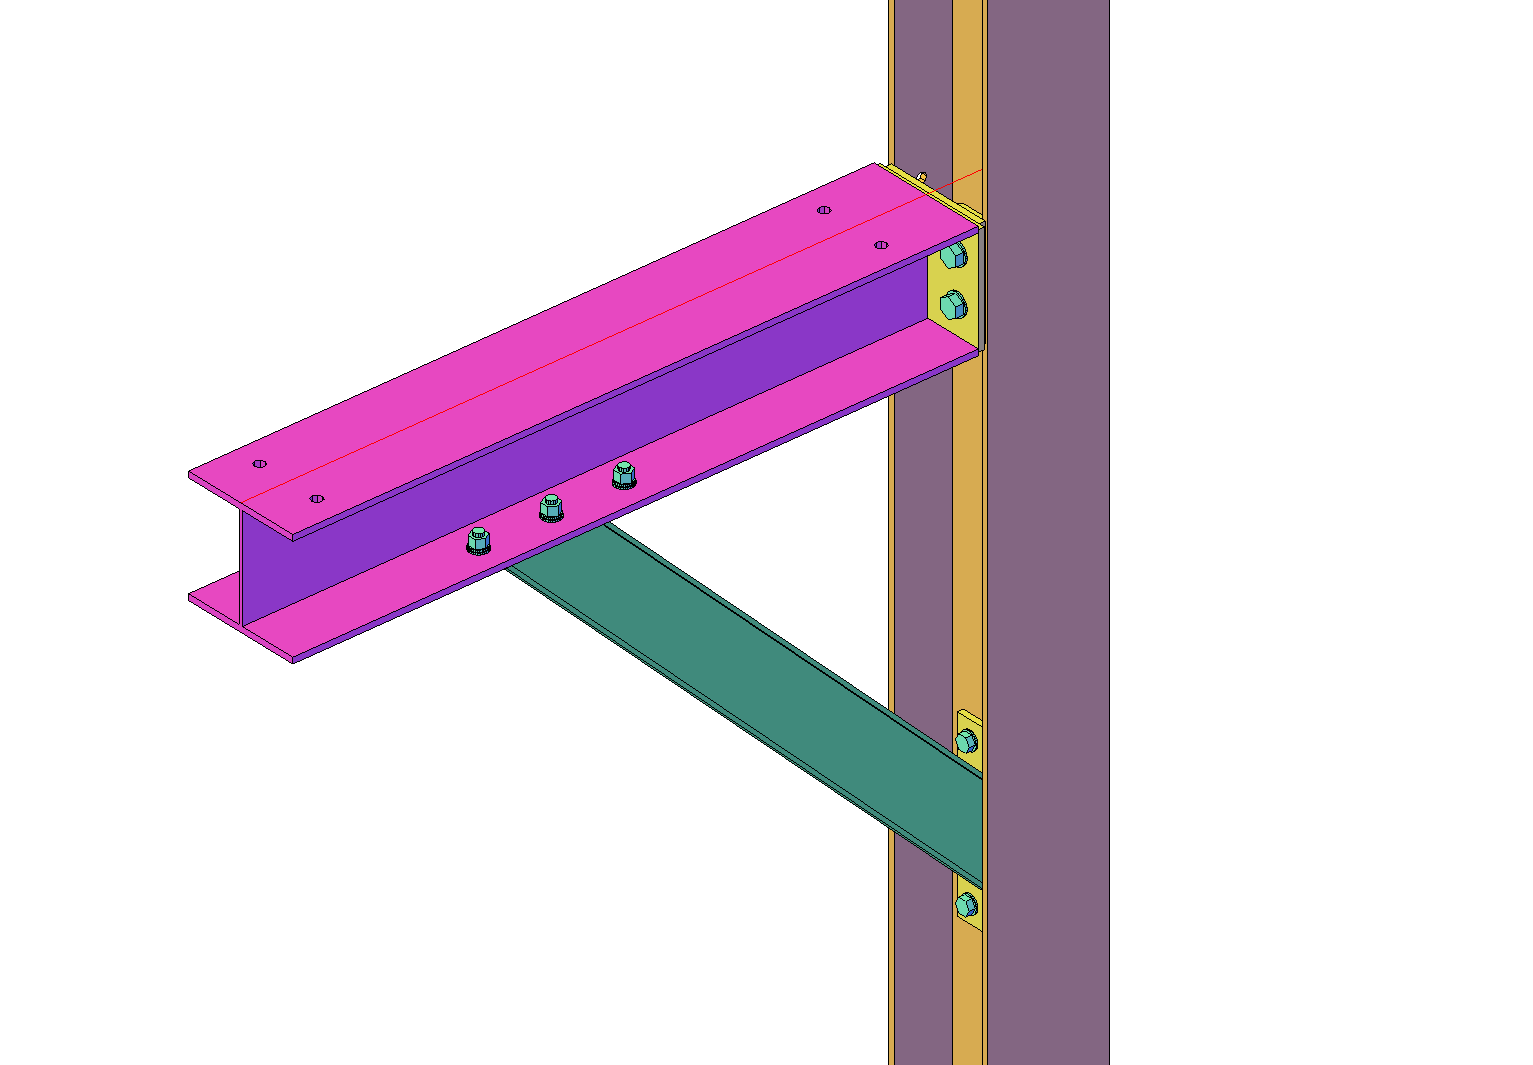
\includegraphics[width=.8\textwidth]{cornerBracing}
\caption{A standard beam and corner bracing connected to a column}\label{fig:cornerBracing}
\end{figure}

\subsection{Mounting conveyors and machines}
Whenever possible UNP and angle is used to mount the conveyors and machines. Folded plate is used when the other options are deemed not possible or practical.\\
Mounting profiles on conveyors and other options have to be present in the sales models, to avoid any mistakes or misconceptions.\\

\newpage 
% If ONLY bollegraaf platforms are used, make sure to turn UNPPlatform off
% !!If visitor platforms are used, UNP Platform needs to be on as well!!
\includeversion{UNPPlatform}
%\excludeversion{UNPPlatform}
\includeversion{visitorsPlatform}
%\excludeversion{visitorsPlatform}
\section{Platforms, railings and stairs}

The standard platform used is a Bollegraaf design. The platforms are placed in Inventor, and no drawings are provided by Tebulo. Bolts are placed in the correct locations in the steel construction.

\begin{UNPPlatform}

Tebulo designed platforms are made out of UNP 160. To join the perpendicular UNP profiles, plates are welded in between the two, as shown in Figure \ref{fig:platformInternally}. When profiles are joined in the corner, the gap is bridged with a bigger plate as shown in Figure \ref{fig:platformCorner}.\\


\begin{minipage}[b]{.47\linewidth}
	\centering
	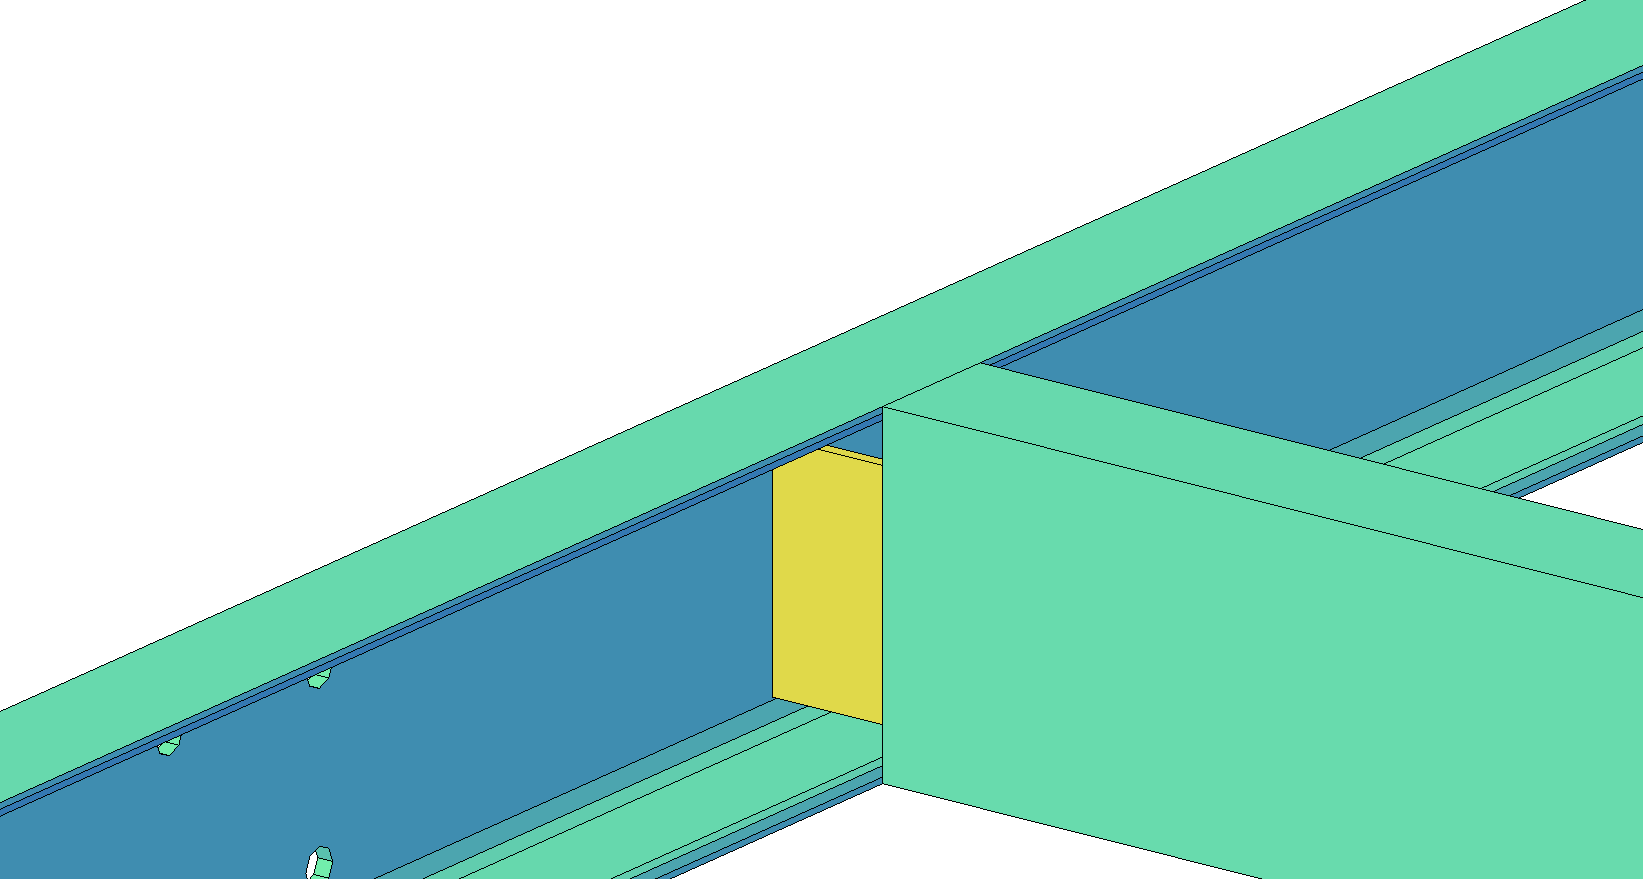
\includegraphics[width=\textwidth]{platformInternally}
	\captionof{figure}{The plates to connect internal perpendicular profiles in the platforms}\label{fig:platformInternally}
\end{minipage}
\qquad
\begin{minipage}[b]{.47\linewidth}
	\centering
	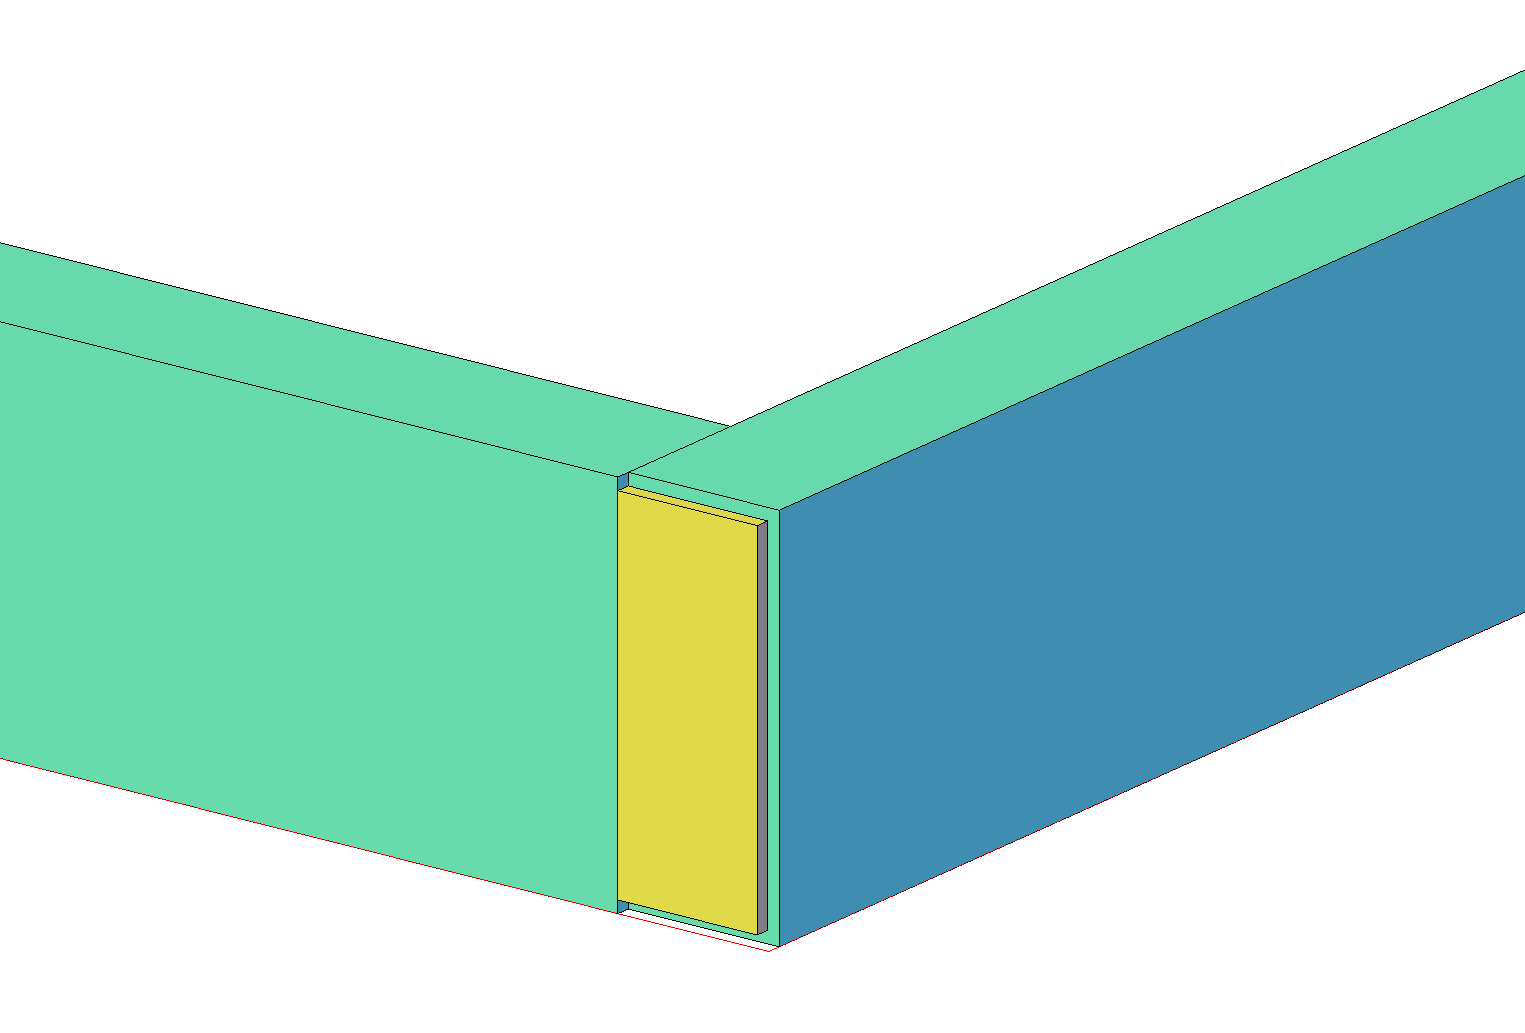
\includegraphics[width=\textwidth]{platformCorner}
	\captionof{figure}{The plates to connect UNP profiles in the platform corners}\label{fig:platformCorner}
\end{minipage}
%\vspace*{.5cm}


The platforms have hoisting eyes welded to the frame to lift them in place, as seen in Figure \ref{fig:platformHoisting}. The left plate is part of the handrail and kickplate. The full handrail can be seen in Figure \ref{fig:handrail}. The handrail is a design of Bollegraaf, and implemented by Tebulo.\\


\begin{minipage}[b]{.47\linewidth}
	\centering
	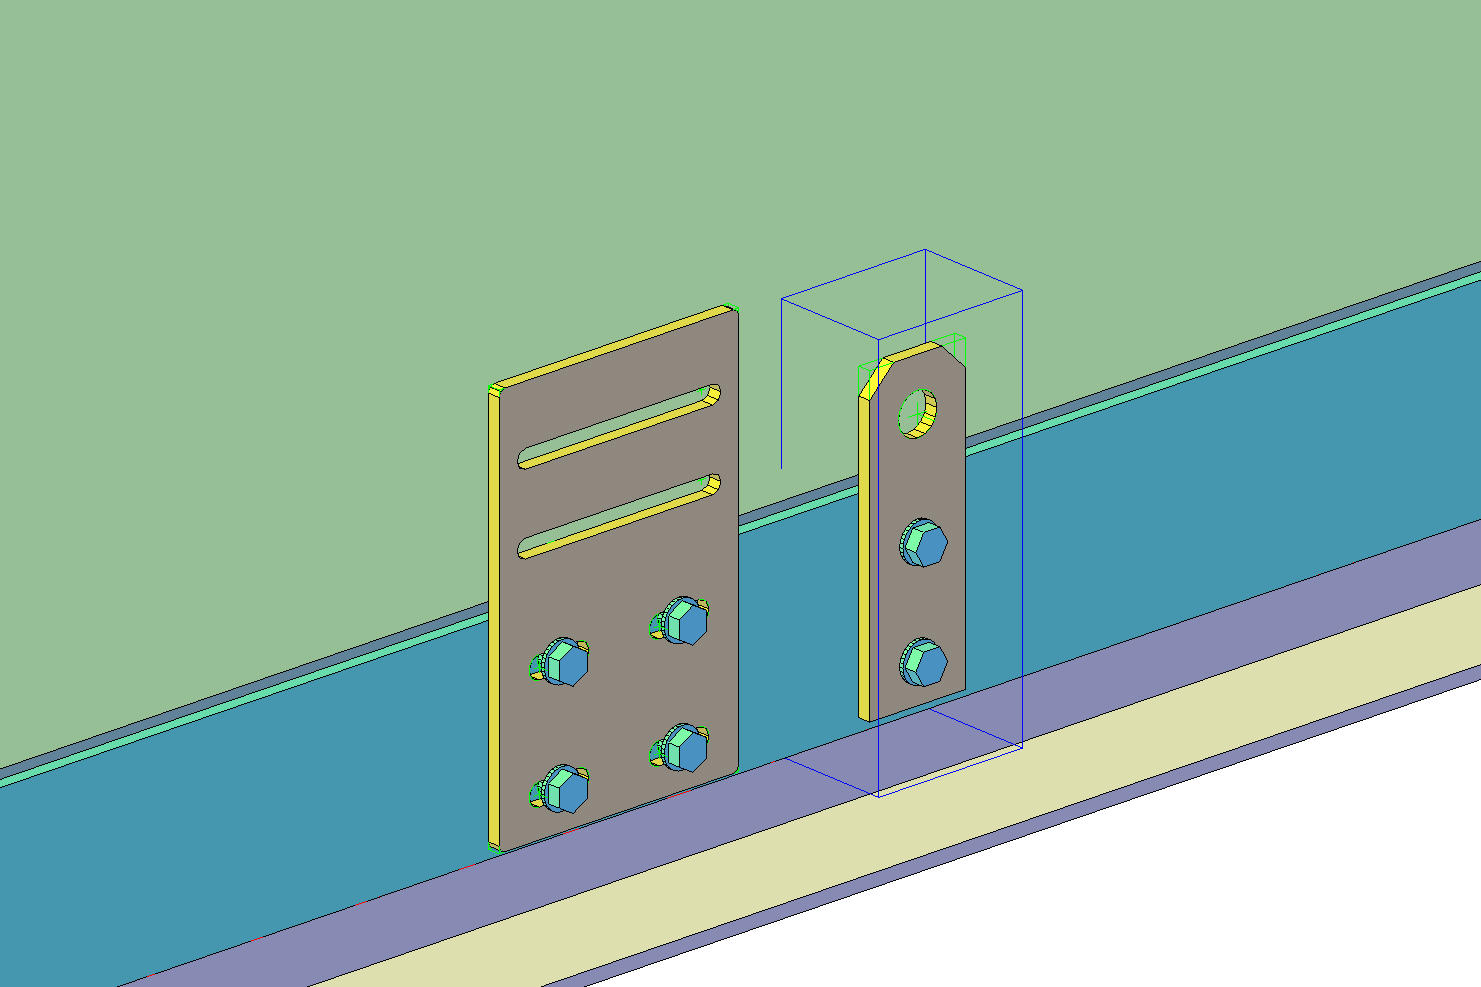
\includegraphics[width=\textwidth]{platformHoistingKickPlates}
	\captionof{figure}{A plate that serves as mounting point for the handrail and kickplate (left). The plates to hoist the platforms into place (Right)}\label{fig:platformHoisting}
\end{minipage}
\qquad
\begin{minipage}[b]{.47\linewidth}
	\centering
	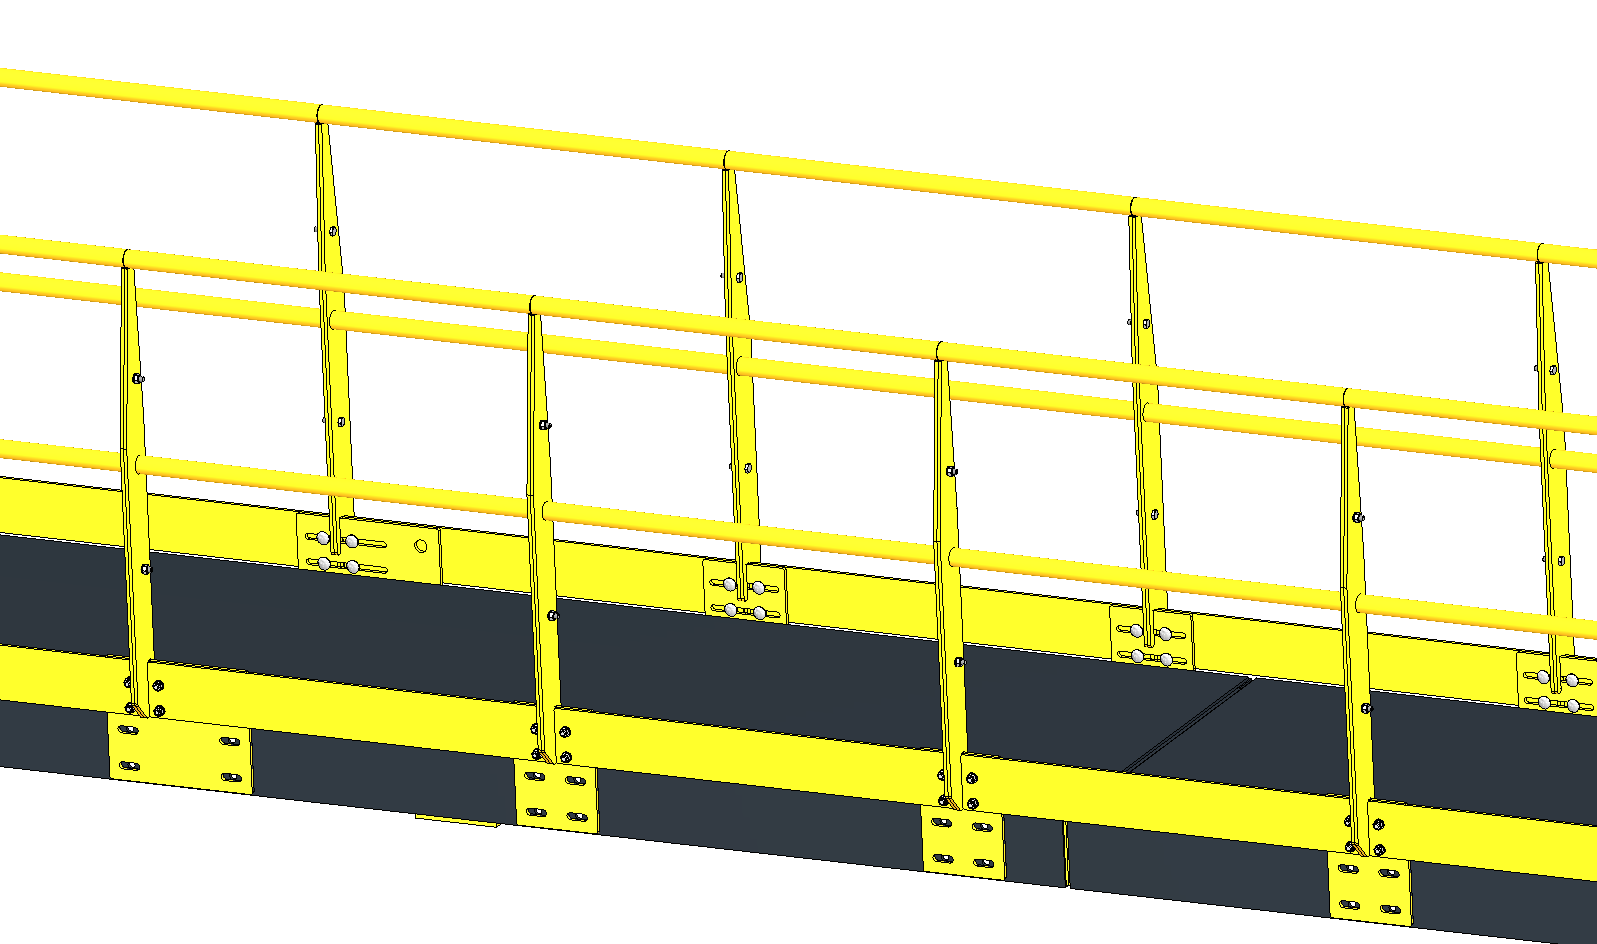
\includegraphics[width=\textwidth]{handrail}
	\captionof{figure}{The Bollegraaf handrail that is mounted on the UNP platforms}\label{fig:handrail}
\end{minipage}
\vspace{.5cm}


The grating placed on the platform has a thickness of 6mm, and is places 10mm from the edges. Furthermore space is reserved for machines and walkways wherever possible. \\
\end{UNPPlatform} \begin{visitorsPlatform}
If visitor platforms are present, they are constructed out of UNP 160 as well. This follows the same method of construction as the UNP platform, but has more requirements. These requirements follow either from \norm\ or agreements with Bollegraaf. These requirements in this project consist of a minimum width of 1.4m, and a different handrail with the bottom part closed off as seen in Figure \ref{fig:visitorPlatform}.

\begin{figure}[H]
\centering
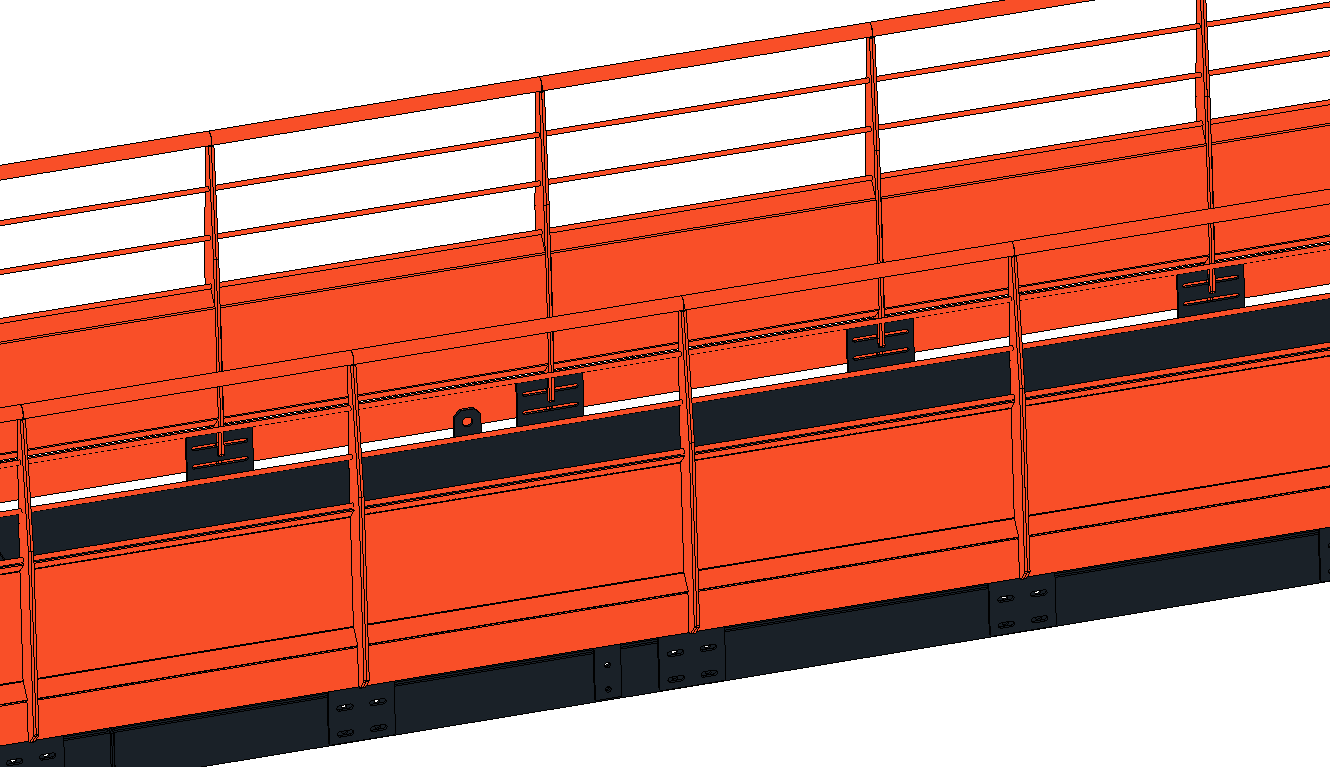
\includegraphics[width=.6\textwidth]{visitorPlatform}
\caption{The handrail used for visitor platforms}\label{fig:visitorPlatform}
\end{figure}

\end{visitorsPlatform}


\newpage
\section{Calculations}
The entire steel construction including the baseplates is calculated according to \norm .\\
To determine if a seismic calculation has to be done for this project, \norm\ will be consulted. Whichever class of calculation is specified by \norm\ shall be followed.\\
\begin{itemize}

\item	Since the conveyors are Bollegraaf's design, the connections, stiffness and deformation of said conveyors is not calculated or considered in the design.
\item	Since the platforms are provided by Bollegraaf, they are not calculated, weights and loads due to the platforms however, are taken into account.
\item	The structural integrity of the concrete floor due to the steel support construction is not calculated.
\item	The act of connecting additional structure or equipment to the structures provided in this report will require a new calculation, and invalidates the results from this report.
\item	If the construction is realised differently from the design of Tebulo, no guarantees can be given about the integrity of the structure.
\item	As long as there are still unreleased items in the project, all given reaction forces, floor loads or other are preliminary, and no conclusions should be drawn from these values.
\end{itemize}



%\newpage
% Only turn on chapter 6 if there are drawings that need to be included. This will usually not be the case.
%\section{Drawings}

\begin{figure}[H]
\centering
\includegraphics[width=.9\textwidth]{PlatformDrawing}
\caption{An example how the platform drawings will be delivered}\label{fig:PlatformDrawing}
\end{figure}

\begin{figure}
\centering
\includegraphics[width=.9\textwidth]{HandrailDrawing}
\caption{An example how the handrail drawings will be delivered}\label{fig:HandrailDrawing}
\end{figure}

\end{document}
